\chapter{Experimental Evaluation}
\label{chap:evaluation}

\section{Main RT-DETR multi-seed study}
\label{sec:rtdetr-main-results}

\subsection{Raw and aggregate VIS+IR results}

All thirty training runs completed the fixed ten-epoch protocol and produced a
final \texttt{latest} checkpoint. \Cref{tab:rtdetr-raw} reports the primary
VIS+IR \mapfifty{} result for every experimental unit.

\begin{table}[htbp]
  \centering
  \caption{Final RT-DETR VIS+IR \mapfifty{} by paired training seed.}
  \label{tab:rtdetr-raw}
  \begin{adjustbox}{max width=\textwidth}
  \begin{tabular}{ccccccc}
    \toprule
    Seed & Base & FAM & FAM + IR Dropout & FAM + SSJ & Identity DCNv2 & Grid Sample \\
    \midrule
    40 & 0.2566 & 0.3783 & 0.4087 & 0.3663 & 0.4336 & 0.4050 \\
    41 & 0.4029 & 0.4335 & 0.3234 & 0.3734 & 0.2113 & 0.3483 \\
    42 & 0.2958 & 0.3129 & 0.4452 & 0.3528 & 0.2926 & 0.4083 \\
    43 & 0.3476 & 0.3964 & 0.3986 & 0.4030 & 0.2860 & 0.3326 \\
    44 & 0.2372 & 0.3690 & 0.3598 & 0.3792 & 0.4162 & 0.3564 \\
    \bottomrule
  \end{tabular}
  \end{adjustbox}
\end{table}

The aggregate distributions in \Cref{tab:rtdetr-aggregate} show why a single
run is insufficient. Identity DCNv2 ranges from 0.2113 to 0.4336, and the
highest value of several individual seeds belongs to a configuration that is
not best on average or consistently paired with the reference.

\begin{table}[H]
  \centering
  \caption{Aggregate final RT-DETR VIS+IR \mapfifty{}. Standard deviations are
  sample standard deviations across five checkpoints.}
  \label{tab:rtdetr-aggregate}
  \begin{adjustbox}{max width=\textwidth}
  \begin{tabular}{lrrrrr}
    \toprule
    Configuration & Mean & Median & SD & Min--max & 95\% CI of mean \\
    \midrule
    Base & 0.3080 & 0.2958 & 0.0677 & 0.2372--0.4029 & 0.2239--0.3921 \\
    FAM & 0.3780 & 0.3783 & 0.0440 & 0.3129--0.4335 & 0.3234--0.4326 \\
    FAM + IR Dropout & \textbf{0.3871} & 0.3986 & 0.0469 & 0.3234--0.4452 & 0.3289--0.4453 \\
    FAM + SSJ & 0.3749 & 0.3734 & \textbf{0.0185} & 0.3528--0.4030 & 0.3519--0.3980 \\
    Identity DCNv2 & 0.3280 & 0.2926 & 0.0943 & 0.2113--0.4336 & 0.2109--0.4451 \\
    Grid Sample & 0.3701 & 0.3564 & 0.0345 & 0.3326--0.4083 & 0.3273--0.4129 \\
    \bottomrule
  \end{tabular}
  \end{adjustbox}
\end{table}

FAM increases mean \mapfifty{} over Base RT-DETR by 0.0700 and wins in all five
paired seeds. Its mean COCO mAP also increases from
\(0.1059\pm0.0243\) to \(0.1351\pm0.0096\), mAP@75 from
\(0.0474\pm0.0128\) to \(0.0692\pm0.0043\), and mAR@100 from
\(0.2474\pm0.0302\) to \(0.2798\pm0.0141\). The direction is therefore not
limited to the primary IoU threshold.

\begin{figure}[H]
  \centering
  \thesisimage[0.95\textwidth]{images/rtdetr_final_paired_map50.pdf}{Paired-seed plot for the six final RT-DETR configurations.}
  \caption{Final RT-DETR VIS+IR \mapfifty{} from the \texttt{latest}
  checkpoints. Panel A connects Base and FAM runs initialized with the same
  training seed; FAM wins all five pairs. Panel B reports, for each seed, the
  difference between a variant and standard FAM, with black bars denoting
  paired means. Each seed-specific run/checkpoint is an experimental unit;
  points are not repeated measurements of one checkpoint.}
  \label{fig:rtdetr-paired-results}
\end{figure}

\subsection{Paired contrasts and model selection}

\Cref{tab:rtdetr-contrasts} compares FAM with Base RT-DETR and compares each FAM
regularization or ablation with the standard FAM. With five pairs, the tests
and intervals are exploratory and are not used as a binary decision rule.

\begin{table}[htbp]
  \centering
  \caption{Paired VIS+IR \mapfifty{} contrasts. A win means that the first
  configuration exceeds its reference for the same training seed.}
  \label{tab:rtdetr-contrasts}
  \begin{adjustbox}{max width=\textwidth}
  \begin{tabular}{lccccc}
    \toprule
    Contrast & Mean delta & SD delta & 95\% CI & Wins & Paired (t) / Wilcoxon (p) \\
    \midrule
    FAM -- Base & +0.0700 & 0.0531 & [+0.0040,+0.1359] & 5/5 & 0.0421 / 0.0625 \\
    FAM + IR Dropout -- FAM & +0.0091 & 0.0869 & [-0.0988,+0.1171] & 3/5 & 0.8260 / 0.8125 \\
    FAM + SSJ -- FAM & -0.0031 & 0.0369 & [-0.0488,+0.0427] & 3/5 & 0.8617 / 1.0000 \\
    Identity DCNv2 -- FAM & -0.0501 & 0.1170 & [-0.1953,+0.0952] & 2/5 & 0.3928 / 0.6250 \\
    Grid Sample -- FAM & -0.0079 & 0.0724 & [-0.0979,+0.0820] & 2/5 & 0.8192 / 1.0000 \\
    \bottomrule
  \end{tabular}
  \end{adjustbox}
\end{table}

IR Dropout has the highest raw mean, but its mean improvement over FAM is only
0.0091, changes sign across seeds, and has a wide interval. It is not selected
as a reliable improvement. SSJ has the smallest descriptive standard deviation
in the six-configuration campaign but does not increase mean performance. Five
runs are insufficient to infer that it reduces population variance.

Identity initialization does not solve final instability. Grid Sample is close
to standard FAM, but its parameterization is not equivalent to DCNv2: it
predicts one displacement per cell and performs no post-sampling filtering or
channel mixing. Its result supports the relevance of a geometric component,
but does not causally assign all FAM improvement to physical alignment.

The main model for subsequent analysis is therefore standard FAM with DCNv2,
without SSJ and without IR feature dropout. Standard FAM is the only final
configuration that exceeds Base in all five paired seeds. The variants are
compared directly with FAM because those contrasts isolate the effect of the
additional intervention: IR feature dropout does not provide a consistent
increment over FAM despite its higher raw mean.

\subsection{Missing-modality evaluation}

Each final checkpoint was evaluated in VIS, IR, and VIS+IR with a fixed
evaluation seed and Modal Dropout disabled. The aggregate \mapfifty{} results
are reported in \Cref{tab:rtdetr-modalities}.

\begin{table}[htbp]
  \centering
  \caption{Final RT-DETR \mapfifty{} by input condition, mean \(\pm\) sample
  standard deviation across five checkpoints.}
  \label{tab:rtdetr-modalities}
  \begin{tabular}{lccc}
    \toprule
    Configuration & VIS & IR & VIS+IR \\
    \midrule
    Base & 0.1543 \(\pm\) 0.0331 & 0.1567 \(\pm\) 0.0464 & 0.3081 \(\pm\) 0.0677 \\
    FAM & 0.2442 \(\pm\) 0.0307 & 0.2028 \(\pm\) 0.0635 & 0.3780 \(\pm\) 0.0439 \\
    FAM + IR Dropout & 0.2368 \(\pm\) 0.0428 & 0.2079 \(\pm\) 0.0267 & 0.3870 \(\pm\) 0.0466 \\
    FAM + SSJ & 0.2312 \(\pm\) 0.0163 & 0.1794 \(\pm\) 0.0416 & 0.3751 \(\pm\) 0.0185 \\
    Identity DCNv2 & 0.2150 \(\pm\) 0.0561 & 0.1768 \(\pm\) 0.0686 & 0.3281 \(\pm\) 0.0942 \\
    Grid Sample & 0.2614 \(\pm\) 0.0267 & 0.1895 \(\pm\) 0.0211 & 0.3701 \(\pm\) 0.0345 \\
    \bottomrule
  \end{tabular}
\end{table}

VIS+IR exceeds the better single modality of the same checkpoint in all thirty
cases. Depending on the configuration, the mean within-checkpoint margin is
between 0.1067 and 0.1454. This is the most uniform result of the main
campaign: on MtErie, complementary information remains useful even though the
individual modality scores vary substantially.

FAM also improves Base RT-DETR in VIS-only in 5/5 seeds, with a mean delta of
0.0899, and in IR-only in 4/5, with a mean delta of 0.0462. In RT-DETR, a
missing input is zero-filled while both backbones and the FAM path remain in
the model. The unimodal difference therefore measures the robustness of the
complete learned system under missing input, not alignment between two real
signals during that inference.

\section{Mechanistic validation of the FAM}
\label{sec:fam-diagnostics}

\subsection{Diagnostic design}

The main detection result establishes a predictive advantage but does not
identify its mechanism. A frozen diagnostic campaign therefore examined
standard FAM, FAM+SSJ, and Grid Sample for seeds 40--44. For every checkpoint,
ten predefined samples were drawn from MtErie, ten from the FHL training
session, and ten from the Baker training session. Each sample was inspected at
P3, P4, and P5:

\begin{equation}
  3\ \text{configurations}\times5\ \text{seeds}\times
  30\ \text{samples}\times3\ \text{levels}=1,350
\end{equation}

sample--level observations. They are aggregated within each checkpoint before
the five checkpoints are compared.

Forward hooks capture RGB and IR features before FAM, the transformed IR
feature, and the predicted offsets and masks. Offset components are converted
to input-image pixels by multiplying them by the level stride. Feature maps are
projected to three shared PCA components for visualization. These pseudo-colour
maps are abstract feature projections and not registered RGB and thermal images.

\subsection{Offset behavior across levels and seeds}

\Cref{tab:fam-offsets} reports the mean absolute offset component after
averaging the thirty samples within each checkpoint. Standard FAM has nonzero
transformations at P3 and P4 in every seed. Excluding the pathological P5
entry, offset scale varies both by seed and level.

\begin{table}[htbp]
  \centering
  \caption{Mean absolute offset components in input-image pixels. Values are
  aggregated over thirty frozen samples per checkpoint.}
  \label{tab:fam-offsets}
  \begin{adjustbox}{max width=\textwidth}
  \begin{tabular}{llrrr}
    \toprule
    Configuration & Seed & P3 & P4 & P5 \\
    \midrule
    FAM & 40 & 2.69 & 3.23 & 13.69 \\
    FAM & 41 & 3.34 & 7.47 & \textbf{5029.83} \\
    FAM & 42 & 3.48 & 6.32 & 34.20 \\
    FAM & 43 & 3.04 & 3.74 & 14.44 \\
    FAM & 44 & 5.99 & 4.80 & 26.63 \\
    \midrule
    FAM + SSJ & 40 & 4.42 & 9.11 & 34.45 \\
    FAM + SSJ & 41 & 3.45 & 10.71 & 23.42 \\
    FAM + SSJ & 42 & 5.41 & 4.73 & 20.95 \\
    FAM + SSJ & 43 & 5.23 & 6.84 & 18.02 \\
    FAM + SSJ & 44 & 6.17 & 4.18 & 36.85 \\
    \midrule
    Grid Sample & 40 & 1.65 & 2.60 & 25.25 \\
    Grid Sample & 41 & 1.70 & 3.59 & 7.66 \\
    Grid Sample & 42 & 2.08 & 2.89 & 11.65 \\
    Grid Sample & 43 & 2.29 & 4.60 & 15.86 \\
    Grid Sample & 44 & 2.41 & 2.49 & 10.17 \\
    \bottomrule
  \end{tabular}
  \end{adjustbox}
\end{table}

At P3, SSJ increases the mean offset magnitude in all five paired seeds; the
mean difference is \((+1.230\pm1.001)\) input pixels. It also reduces the ratio
of output-to-input spatial variation in all five checkpoints, producing a
smoother transformed feature. P4 offset changes are less consistent, and P5
cannot be paired directly with standard FAM without accounting for the seed-41
collapse. The diagnostic conclusion agrees with the detection result: SSJ
changes the learned module in a repeatable way at P3, but that change does not
improve final detection accuracy.

Grid Sample has smaller and less dispersed P3/P4 offsets. Unlike DCNv2, it
performs only a bilinear warp, without learned post-sampling filtering or
channel mixing. Its output can therefore be interpreted more directly as a
spatially transformed IR feature, whereas the DCNv2 output is a broader
feature-space transformation. Neither operation establishes physical camera
alignment.

\subsection{P5 collapse in seed 41}
\label{sec:p5-collapse}

FAM seed 41 exhibits a complete and repeated P5 degeneration across all thirty
samples and all three sessions. Its mean absolute offset is approximately
5,030 input pixels, orders of magnitude larger than the normal checkpoints.
The transformed IR output has zero spatial standard deviation and equals the
learned DCNv2 bias at every location.

\begin{figure}[p]
  \centering
  \thesisimage[0.9\textwidth]{images/fam_p5_seed41_collapse.png}{Mechanistic diagnostic of the P5 collapse in FAM seed 41.}
  \caption{Mechanistic diagnostic of the collapsed P5 branch in FAM seed 41
  for the prespecified MtErie sample 35. Panels (a)--(c) are pseudo-colour PCA
  projections obtained with a basis shared across the standardized feature
  tensors; panels (d)--(e) are qualitative 50\% blends and are not tensors
  consumed by the detector. Panel (f) summarizes absolute DCNv2 offset
  components in feature-cell coordinates and the modulation-mask statistics.
  The transformed IR feature is spatially constant, while the mean absolute
  offset component corresponds to 5,227 input pixels. These quantities diagnose
  a learned feature-space transformation and must not be interpreted as a
  camera-registration field.}
  \label{fig:fam-p5-collapse}
\end{figure}

The scale anomaly is already present before FAM: mean P5 global standard
deviations are 17.30 for RGB and 20.18 for IR, compared with 0.17--0.69 and
0.056--0.101 in the other seeds. The offset predictor itself has ordinary
weight norms. Its enormous offsets are nearly identical across samples
(correlation above 0.999) and sample outside the feature map, leaving only the
deformable-convolution bias.

The detector nevertheless obtains 0.4335 \mapfifty{}, the highest of the five
FAM checkpoints. High output accuracy therefore does not guarantee that every
internal alignment level behaves sensibly. The main FAM advantage is not
created by the anomaly: after excluding seed 41, FAM still beats Base RT-DETR in
4/4 paired seeds with mean delta (+0.0799).

\subsection{Factorial P3/P4/P5 ablation}

All eight subsets of active FAM levels were evaluated post-hoc in each of the
five trained FAM checkpoints. Bypassing a level replaces its transformed IR
feature with the pre-FAM IR feature. The intervention measures sensitivity of
the trained system; it does not reproduce training a network with that level
absent.

\begin{table}[htbp]
  \centering
  \caption{Post-hoc factorial level ablation. Delta is the paired mean
  difference from the full trained FAM.}
  \label{tab:fam-level-ablation}
  \begin{tabular}{lrrr}
    \toprule
    Active FAM levels & Mean \mapfifty{} & SD & Delta from full \\
    \midrule
    None & 0.2259 & 0.0654 & -0.1521 \\
    P3 & 0.3223 & 0.0660 & -0.0558 \\
    P4 & 0.2396 & 0.0983 & -0.1384 \\
    P5 & 0.2791 & 0.0377 & -0.0989 \\
    P3 + P4 & 0.3221 & 0.0701 & -0.0559 \\
    P3 + P5 & 0.3648 & 0.0503 & -0.0132 \\
    P4 + P5 & 0.2984 & 0.0254 & -0.0796 \\
    P3 + P4 + P5 & \textbf{0.3780} & 0.0440 & 0.0000 \\
    \bottomrule
  \end{tabular}
\end{table}

P3 has the largest and most stable factorial main effect. P5 has a positive
mean effect but high variability, dominated by seed 41. Removing P5 from that
checkpoint reduces \mapfifty{} from 0.4335 to 0.2399. The decoder has adapted
to, or learned to compensate for, the collapsed representation. Static removal
after training is therefore not a repair, and the result does not predict the
score of a newly trained P3+P4-only model.

\subsection{Bounded-offset intervention}
\label{sec:bounded-fam}

The proximal mechanism of the constant output is unbounded sampling far
outside the feature map. A single corrective hypothesis was therefore frozen
before new training. For every raw offset component, the bounded variant uses

\begin{equation}
  \Delta_{\mathrm{eff}}=4\tanh\!\left(\frac{\Delta_{\mathrm{raw}}}{4}\right),
  \label{eq:bounded-offset}
\end{equation}

where the limit is expressed in cells of the current feature level. The
derivative at zero is one, and no gate, normalization, residual connection, or
backbone modification is introduced. The limit of four cells was chosen from
the non-pathological checkpoint distributions before observing the five new
training results.

\begin{table}[htbp]
  \centering
  \caption{Automatic VIS+IR \mapfifty{} for the five bounded-offset runs and
  the corresponding frozen standard-FAM reference.}
  \label{tab:bounded-raw}
  \begin{tabular}{rrrr}
    \toprule
    Seed & Standard FAM & Bounded FAM & Bounded -- standard \\
    \midrule
    40 & 0.3783 & 0.4208 & +0.0426 \\
    41 & 0.4335 & 0.3319 & -0.1015 \\
    42 & 0.3129 & 0.4214 & +0.1085 \\
    43 & 0.3964 & 0.2735 & -0.1229 \\
    44 & 0.3690 & 0.2998 & -0.0692 \\
    \midrule
    Mean \(\pm\) SD & 0.3780 \(\pm\) 0.0440 & 0.3495 \(\pm\) 0.0686 & -0.0285 \\
    \bottomrule
  \end{tabular}
\end{table}

The bounded model wins in only 2/5 seeds and has greater dispersion. Its
standalone modality evaluation obtains
\(0.2252\pm0.0544\) VIS,
\(0.1943\pm0.0272\) IR, and
\(0.3496\pm0.0685\) VIS+IR, all below the standard-FAM means.

The internal intervention nevertheless succeeds. Every observed effective
offset remains below four cells, including a maximum of 3.9915 at P5 seed 41,
and none of the 150 inspected P5 checkpoint--sample cases has a spatially
constant output. Raw offsets would still reach 13.69 cells, showing that the
bound is active. The experiment therefore separates two outcomes: the targeted
failure mode is removed, but detection does not improve. Standard FAM remains
the selected model.

\section{Detection error analysis}
\label{sec:error-analysis}

\subsection{Protocol}

The error analysis compares the five Base RT-DETR and five standard-FAM final
checkpoints on all 708 MtErie frames and 1,770 objects. Predictions are matched
one-to-one to annotations at IoU at least 0.50. The primary evaluation retains
all predictions with confidence at least 0.01, as in the final mAP evaluation.
For the predefined sensitivity analysis, this same prediction set is
additionally thresholded at 0.05, 0.10, 0.25, and 0.50 when reporting
precision, recall, and false positives. These thresholds are not used for model
selection or to select a deployment threshold.

Of the 1,770 objects, 1,451 are COCO-small, 301 medium, and 18 large at the
evaluation resolution. Large-object results are therefore particularly
uncertain.

\subsection{Results across thresholds}

\begin{table}[htbp]
  \centering
  \caption{Paired RT-DETR error behavior across confidence thresholds. Values
  are mean \(\pm\) sample standard deviation over five checkpoints.}
  \label{tab:error-thresholds}
  \begin{adjustbox}{max width=\textwidth}
  \begin{tabular}{rrcccc}
    \toprule
    Threshold & Model & Precision & Recall & FP/image & Non-empty frames with FN \\
    \midrule
    0.01 & Base & 0.0418 \(\pm\) 0.0175 & 0.7677 \(\pm\) 0.0490 & 51.006 \(\pm\) 21.591 & 0.4508 \(\pm\) 0.0777 \\
    0.01 & FAM & 0.0443 \(\pm\) 0.0132 & 0.8044 \(\pm\) 0.0328 & 47.623 \(\pm\) 17.873 & 0.4009 \(\pm\) 0.0524 \\
    0.05 & Base & 0.2713 \(\pm\) 0.0909 & 0.5932 \(\pm\) 0.1134 & 4.844 \(\pm\) 3.199 & 0.6476 \(\pm\) 0.1155 \\
    0.05 & FAM & 0.3010 \(\pm\) 0.0940 & 0.6539 \(\pm\) 0.0972 & 4.336 \(\pm\) 2.191 & 0.5835 \(\pm\) 0.0775 \\
    0.10 & Base & 0.4721 \(\pm\) 0.0923 & 0.4582 \(\pm\) 0.1535 & 1.513 \(\pm\) 1.115 & 0.7466 \(\pm\) 0.1223 \\
    0.10 & FAM & 0.5194 \(\pm\) 0.1148 & 0.5507 \(\pm\) 0.1333 & 1.447 \(\pm\) 0.792 & 0.6554 \(\pm\) 0.0725 \\
    0.25 & Base & 0.7290 \(\pm\) 0.0866 & 0.2340 \(\pm\) 0.1468 & 0.249 \(\pm\) 0.218 & 0.8682 \(\pm\) 0.0879 \\
    0.25 & FAM & 0.7715 \(\pm\) 0.0742 & 0.3330 \(\pm\) 0.1506 & 0.276 \(\pm\) 0.168 & 0.7858 \(\pm\) 0.0525 \\
    0.50 & Base & 0.9140 \(\pm\) 0.0536 & 0.1088 \(\pm\) 0.0705 & 0.029 \(\pm\) 0.033 & 0.9257 \(\pm\) 0.0588 \\
    0.50 & FAM & 0.9350 \(\pm\) 0.0504 & 0.1627 \(\pm\) 0.0663 & 0.036 \(\pm\) 0.037 & 0.8790 \(\pm\) 0.0359 \\
    \bottomrule
  \end{tabular}
  \end{adjustbox}
\end{table}

Recall is the most consistent difference. FAM is better in 5/5 seeds at
thresholds 0.10, 0.25, and 0.50. At 0.25, recall increases from 0.2340 to
0.3330, a mean paired gain of 0.0990, and the fraction of non-empty frames with
at least one missed target decreases by 0.0824.

The gain is not limited to the 18 large objects. At threshold 0.25, mean recall
increases by 0.0815 for small and 0.1781 for medium targets. False positives do
not improve uniformly: FAM produces slightly fewer on average at low
thresholds and slightly more at 0.25 and 0.50, with signs that vary across
seeds.

\begin{figure}[htbp]
  \centering
  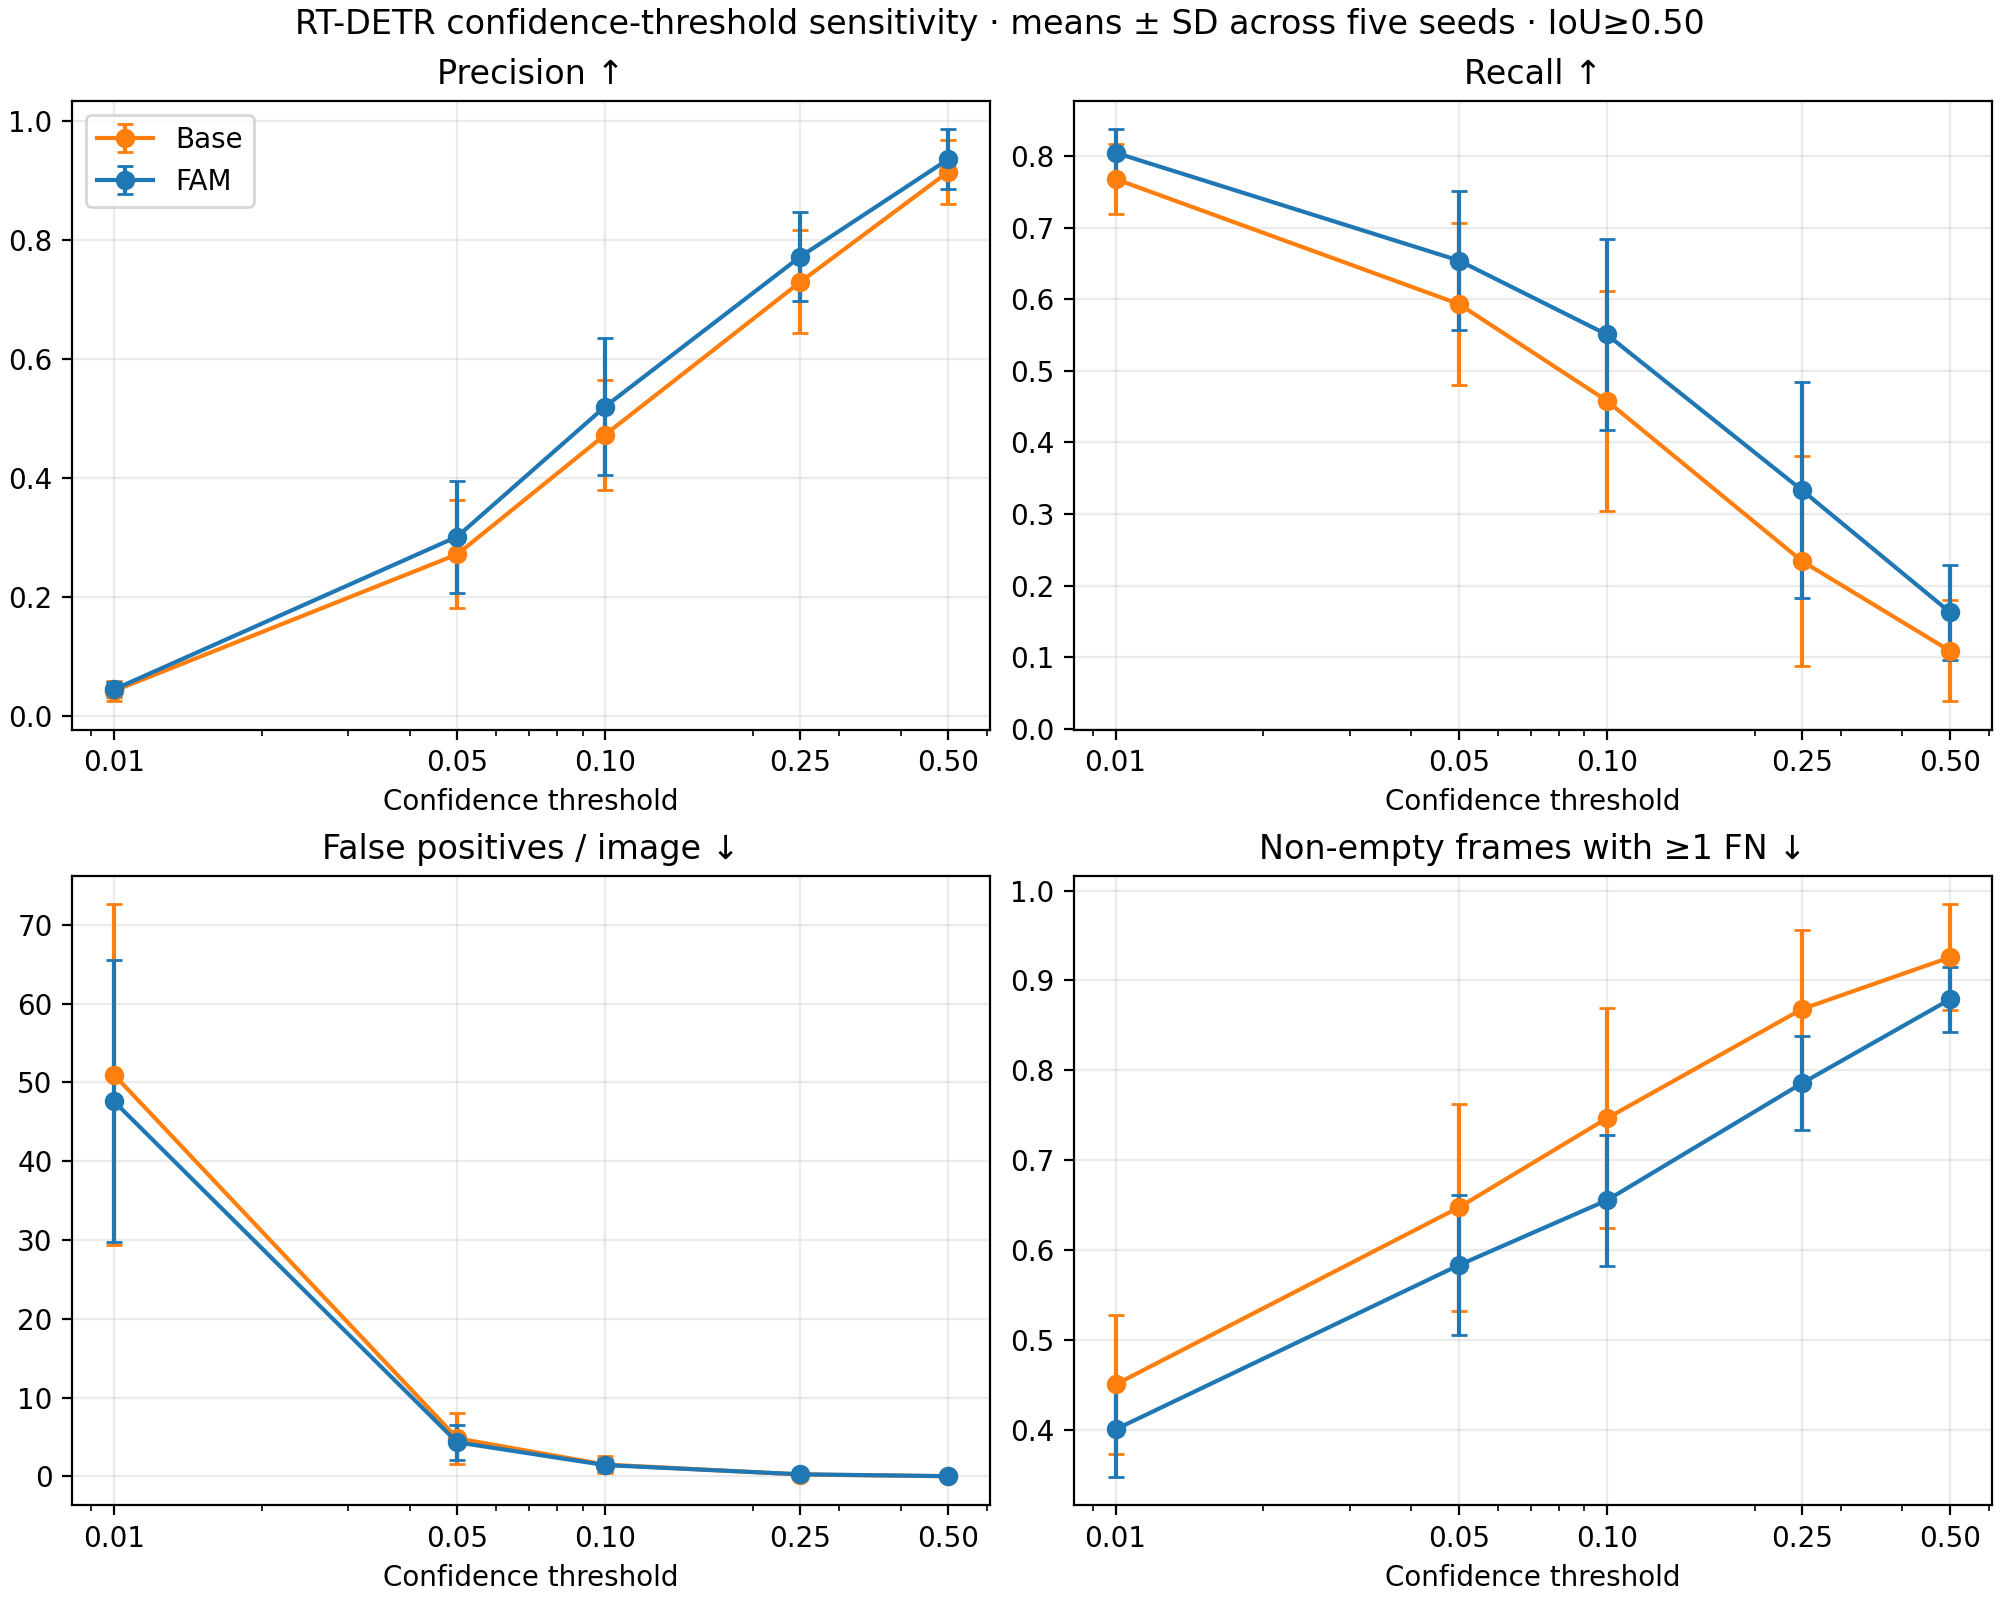
\includegraphics[width=0.95\textwidth]{images/rtdetr_additive_fam_threshold_sensitivity.png}
  \caption{Sensitivity of precision, recall, false positives per image, and
  non-empty frames with a false negative to the five predefined confidence
  thresholds. Error bars are sample standard deviations across checkpoints.}
  \label{fig:error-threshold-sensitivity}
\end{figure}

At threshold 0.01, both configurations generate approximately 48--51 false
positives per image. This threshold is appropriate for collecting a broad set
of candidates for AP computation but is not an operational alarm threshold.

\subsection{Qualitative examples}

The qualitative manifest was built from ground-truth annotations before
inference. For each of the three MtErie sequences, it selects one frame with a
small target and one empty frame. Seed 43 is used because its FAM--Base
\mapfifty{} difference equals the median of the five paired differences; it is
neither the best nor worst pair.

\begin{figure}[H]
  \centering
  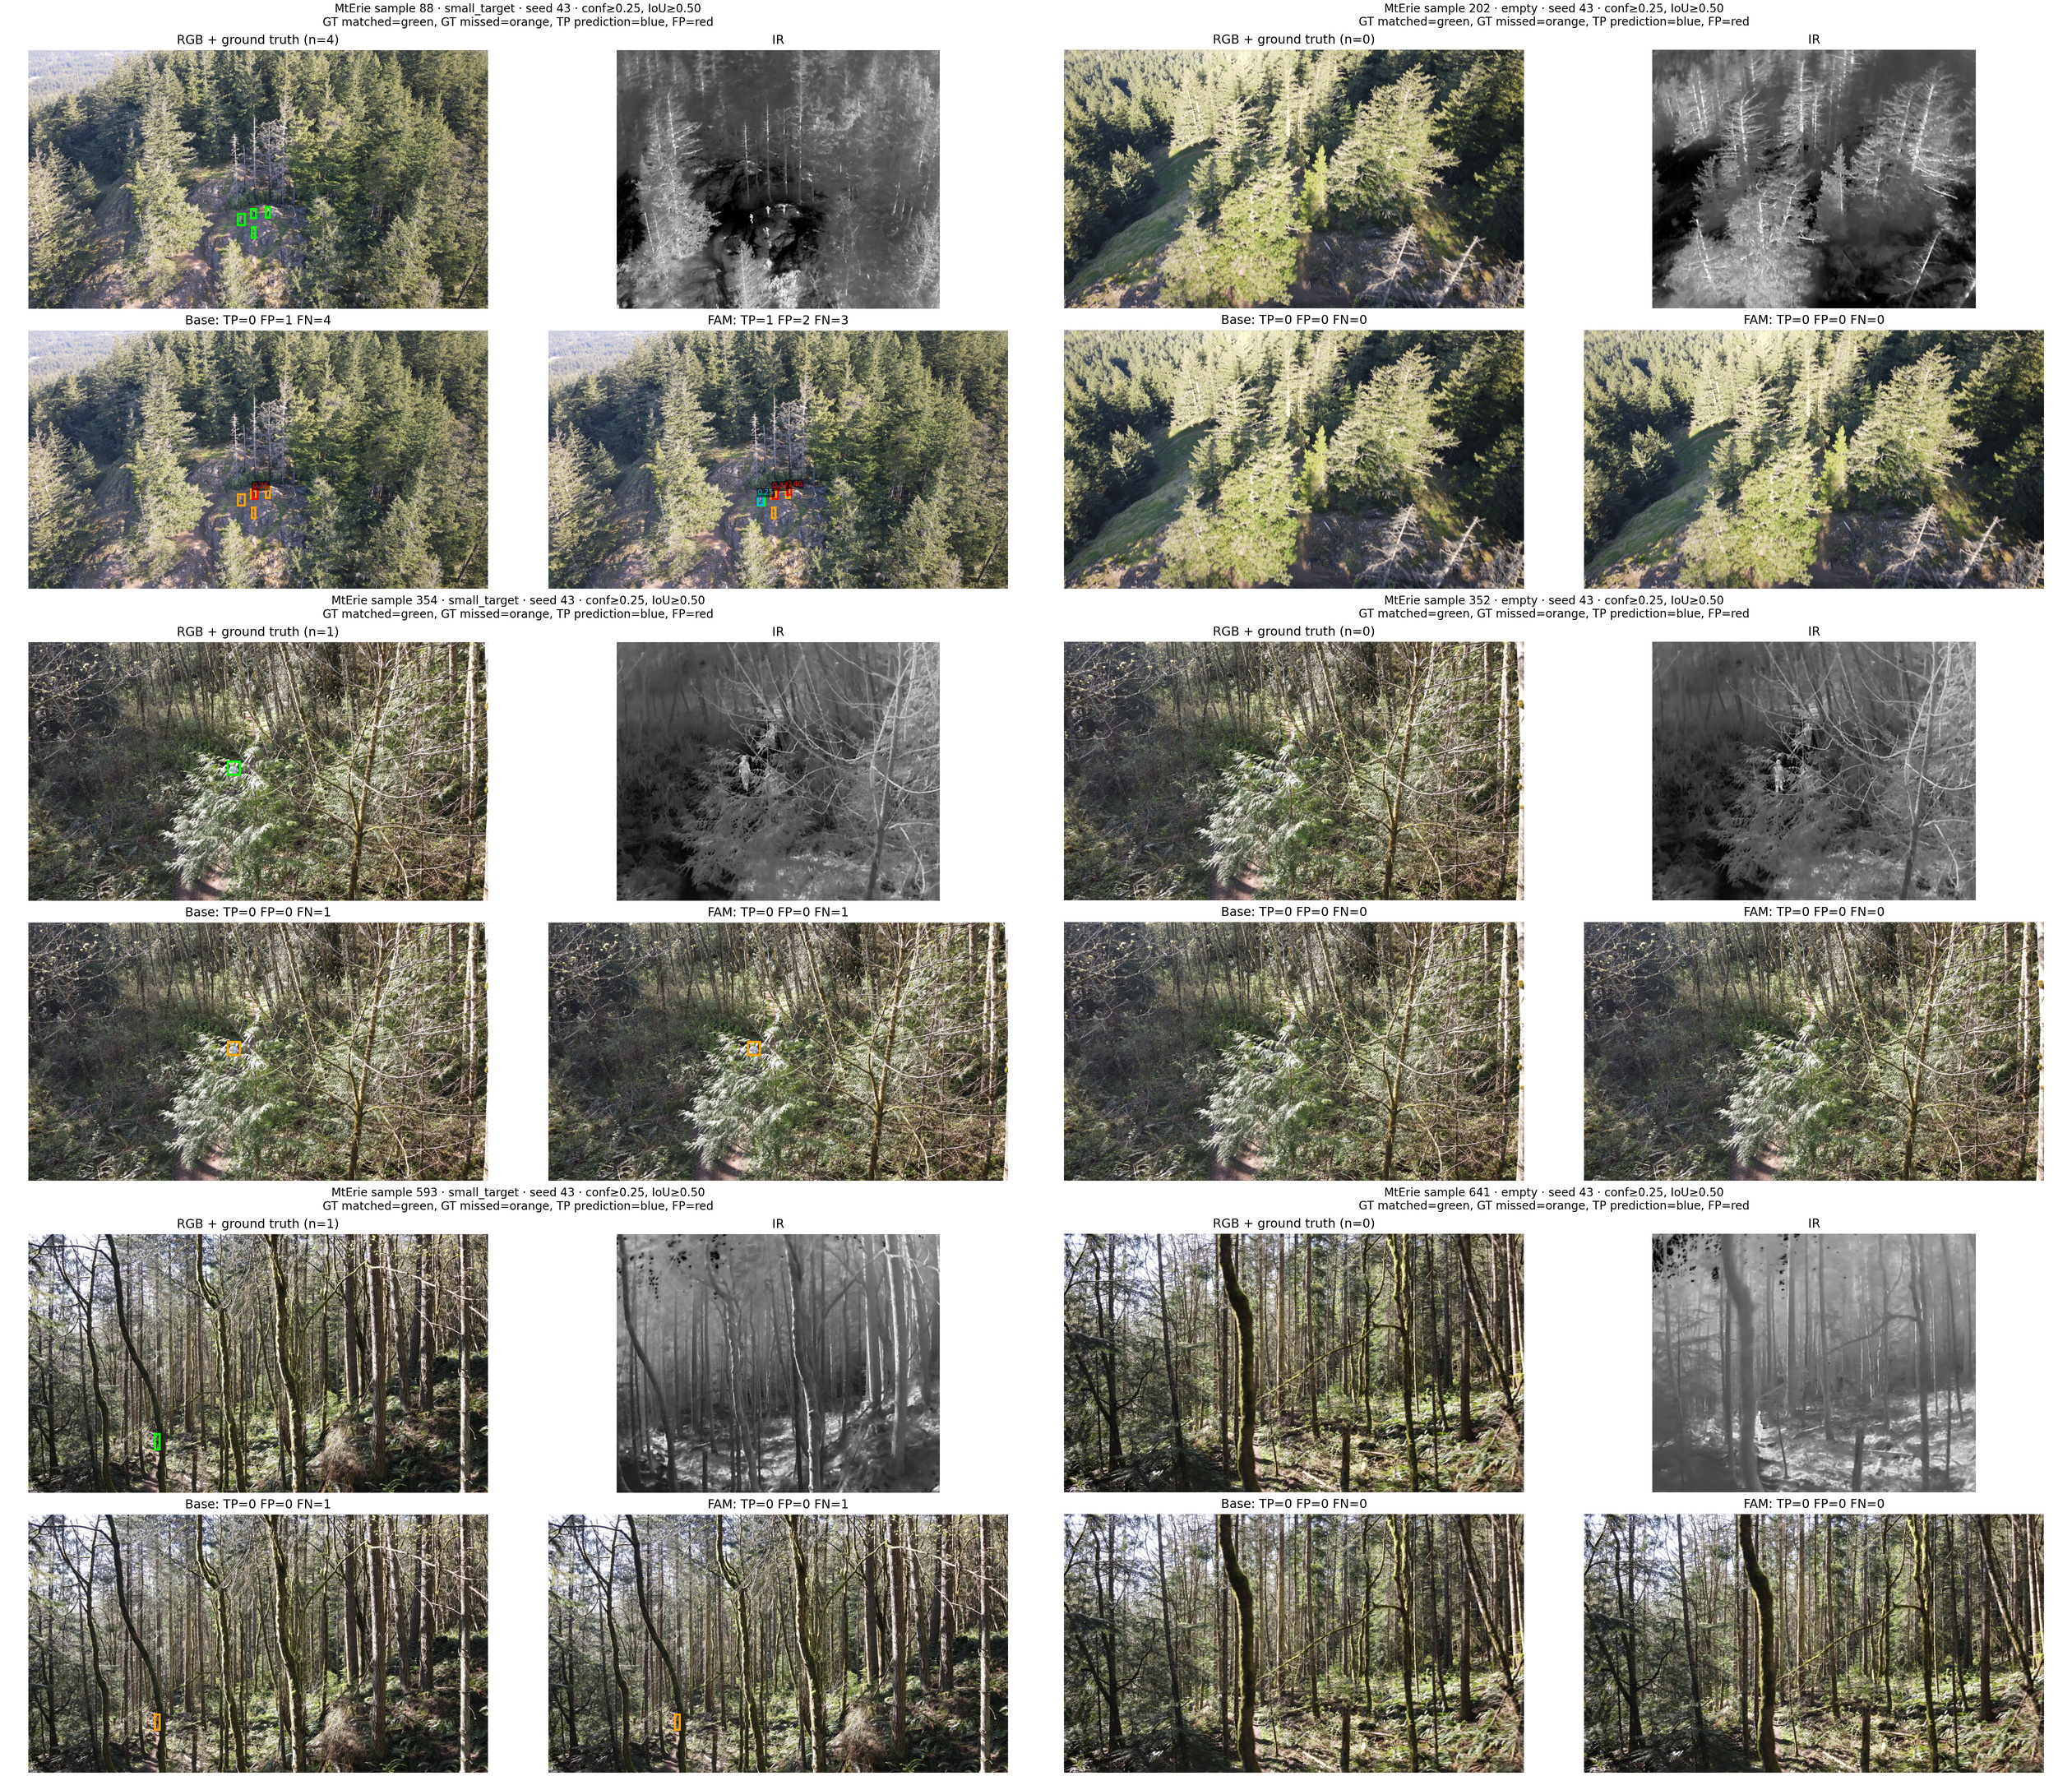
\includegraphics[width=\textwidth]{images/rtdetr_error_qualitative_conf_025.jpg}
  \caption{Predefined qualitative examples at confidence 0.25. Each row
  contains one small-target frame and one empty frame from a MtErie sequence.
  The same frames and display rules are used for Base RT-DETR and FAM. These
  examples illustrate, but do not replace, the aggregate analysis.}
  \label{fig:error-qualitative-025}
\end{figure}

The corresponding threshold-0.01 montage is retained in the appendix because
the large number of low-confidence boxes makes it difficult to read. In the
three predefined small-target frames at 0.25, FAM recovers one target missed by
Base RT-DETR in one frame; both models miss the targets in the other two. No
general conclusion is drawn from these six examples.

\section{Carnation scale-mismatch stress test}
\label{sec:carnation}

\subsection{Frozen design}

Carnation contains a paired visual and thermal acquisition with a substantially
stronger scale mismatch than the main splits. Its protocol was frozen before
inference and admits only the five final Base RT-DETR and five final FAM
checkpoints. The intersection of frame identifiers contains 739 examples.
Each checkpoint is evaluated in VIS+IR, VIS, and IR, yielding thirty
evaluations without training, tuning, checkpoint selection, or threshold
selection.

Carnation is a deliberately difficult single acquisition. It is not a
representative sample of SAR domains, a new validation set, or an estimate of
general domain generalization.

\subsection{Results}

\begin{table}[htbp]
  \centering
  \caption{Carnation \mapfifty{} across five frozen checkpoints.}
  \label{tab:carnation-results}
  \begin{tabular}{lrrrr}
    \toprule
    Input & Base RT-DETR & FAM & Mean paired delta & FAM wins \\
    \midrule
    VIS+IR & 0.1445 \(\pm\) 0.0709 & 0.2408 \(\pm\) 0.0380 & +0.0962 & 4/5 \\
    VIS & 0.1555 \(\pm\) 0.0669 & 0.3196 \(\pm\) 0.0518 & +0.1641 & 5/5 \\
    IR & 0.1288 \(\pm\) 0.0776 & 0.0979 \(\pm\) 0.0652 & -0.0308 & 1/5 \\
    \bottomrule
  \end{tabular}
\end{table}

FAM is more tolerant than Base RT-DETR in the fusion condition, with a mean gain
of 0.0962 and four paired wins. This is not sufficient to make fusion the best
input condition. For the FAM checkpoints, VIS-only exceeds VIS+IR in all five
seeds by a mean of 0.0789. Adding the strongly mismatched IR signal is therefore
harmful relative to the available visible stream even after FAM transformation.

\begin{figure}[htbp]
  \centering
  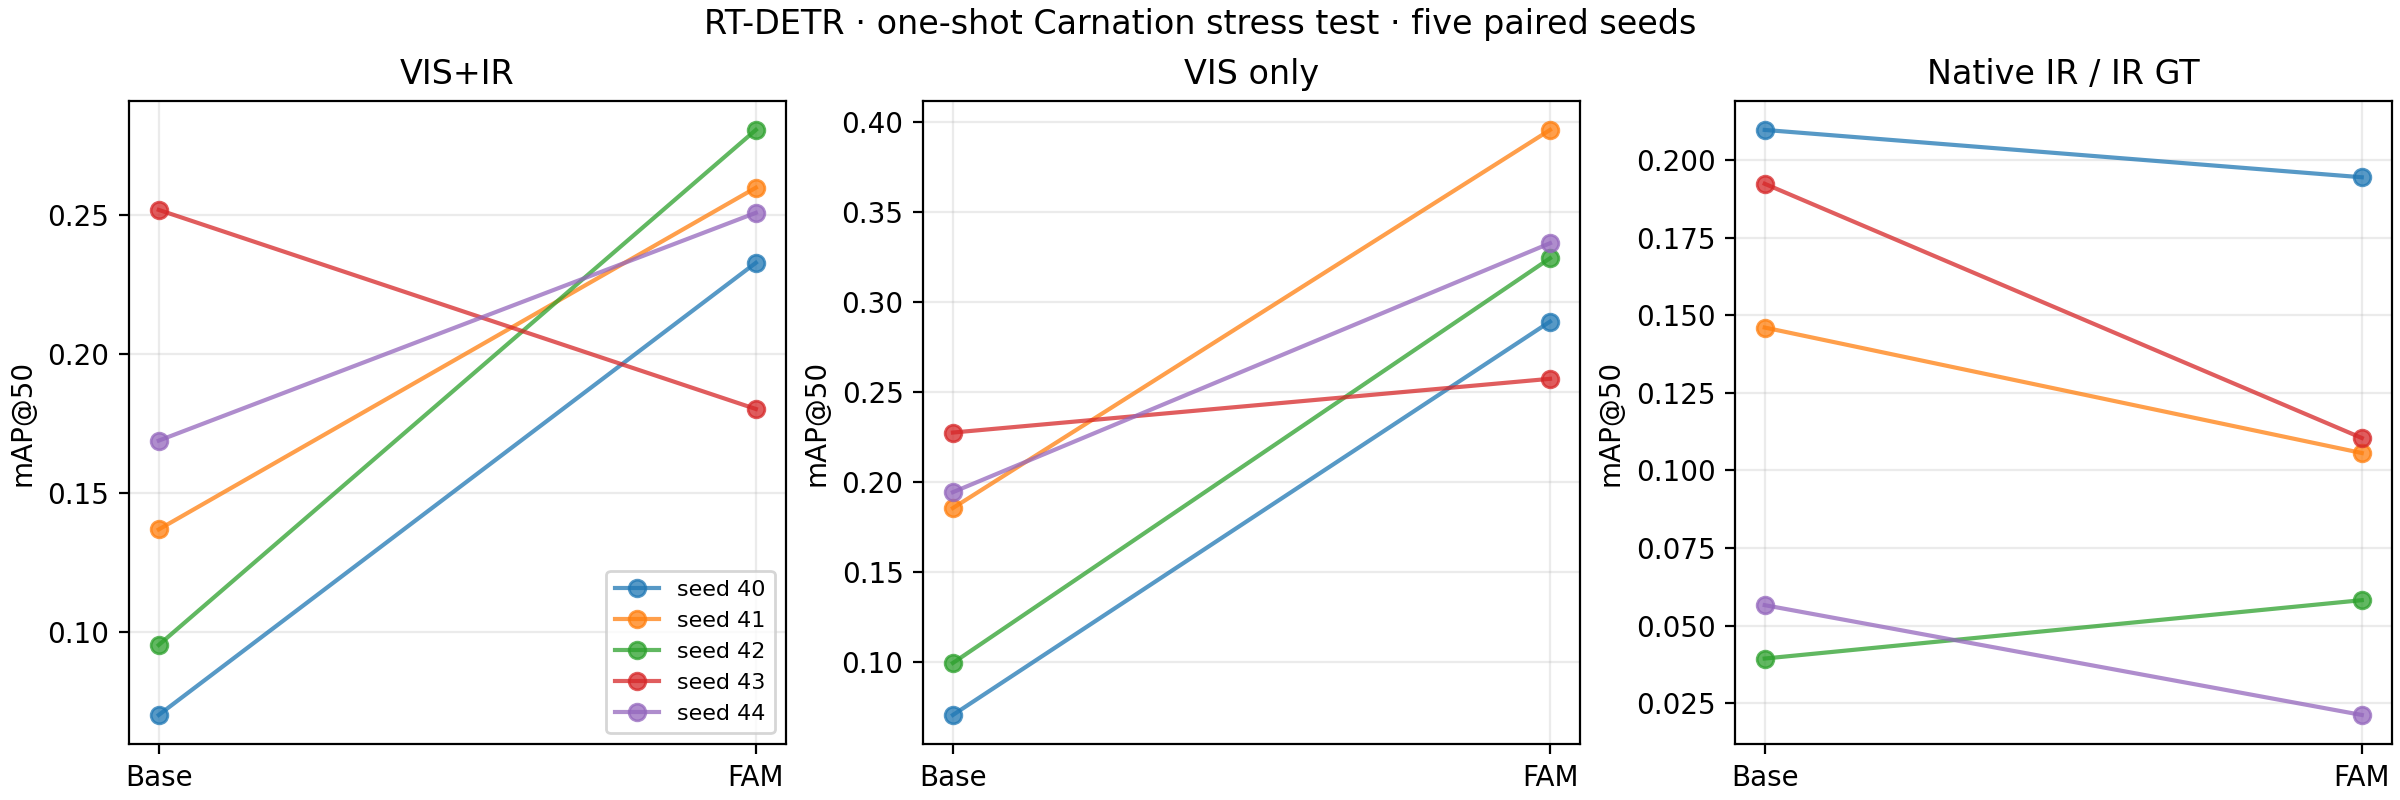
\includegraphics[width=\textwidth]{images/rtdetr_carnation_paired_map50.png}
  \caption{Paired Carnation results for the three modality conditions. The
  stress test shows partial damage mitigation by FAM, not correction of the
  severe mismatch.}
  \label{fig:carnation-paired}
\end{figure}

The result also bounds the internal MtErie finding that VIS+IR was always
better than the strongest single modality. That conclusion is stable within
the main benchmark but does not survive this extreme acquisition.

\section{Computational cost}
\label{sec:compute}

The compute comparison uses the seed-43 Base RT-DETR and FAM RT-DETR
checkpoints, chosen in advance as the same typical pair used for qualitative
illustrations. Each
configuration is measured in three isolated processes on an NVIDIA GeForce RTX
4070 Laptop GPU with PyTorch 2.4.0, CUDA 12.1, batch size one, FP32 input of
\(640\times640\), thirty warm-up iterations, and one hundred timed forward
passes per trial. TF32, autocast, preprocessing, and postprocessing are
excluded.

\begin{table}[htbp]
  \centering
  \caption{RT-DETR detector-only computational benchmark. The operation count is a
  proxy and the latency uncertainty is the sample standard deviation across
  three trial means.}
  \label{tab:compute-results}
  \begin{adjustbox}{max width=\textwidth}
  \begin{tabular}{lrrrrr}
    \toprule
    Model & Parameters & Proxy GFLOPs & Latency & Throughput & CUDA peak \\
    \midrule
    Base & 66.20 M & 208.37 & 66.91 \(\pm\) 0.30 ms & 14.95 image/s & 436.26 MiB \\
    FAM & 117.49 M & 304.54 & 78.87 \(\pm\) 0.37 ms & 12.68 image/s & 712.18 MiB \\
    \bottomrule
  \end{tabular}
  \end{adjustbox}
\end{table}

Relative to Base RT-DETR, FAM adds 77.5\% parameters, 46.2\% proxy computation,
17.9\% detector latency, and 275.92 MiB of total peak CUDA memory. The proxy
adds an analytical dense-convolution equivalent for DCNv2 because the profiler
does not count that operator fully; it still omits parts of bilinear sampling,
mask application, and sigmoid evaluation. Measured latency is therefore the
more operational quantity, while remaining specific to this GPU and detector
scope.

The FAM improvement is not computationally free. Deployment decisions must
weigh its recall and \mapfifty{} gains against memory, throughput, energy, and
the unmeasured cost of the full UAV pipeline.

\section{Architectural transferability to YOLOv10}
\label{sec:yolo-transfer}

\subsection{Dual-backbone architecture}

The YOLOv10-s transfer model receives a four-channel paired tensor and splits
it into a three-channel RGB stream and one-channel IR stream. Two independent
backbones produce P3, P4, and P5 features at strides 8, 16, and 32. The
Base configuration sums each pair; the FAM configuration applies the same
standard DCNv2 module to IR before addition. The resulting features enter the
shared YOLOv10 FPN/PAN neck and detection head.

Missing modalities are implemented through feature gating. During training,
one branch or both are selected with probabilities 0.2/0.2/0.6. In standalone
VIS or IR evaluation, the excluded backbone is not executed and FAM is
bypassed because a paired reference is unavailable. Unimodal differences
therefore reflect how training with FAM shaped the remaining weights, not a
direct alignment operation at inference.

\begin{figure}[H]
  \centering
  \thesisimage[0.92\textwidth]{images/yolov10_dual_backbone_fam.pdf}{Diagram of the implemented YOLOv10 dual-backbone Base and FAM configurations.}
  \caption{Implemented YOLOv10-s transfer architecture. The controlled
  comparison changes the P3/P4/P5 fusion operation while retaining the dual
  backbones, feature gating, FPN/PAN neck, detection head, and final protocol.
  The FAM operation is the same as the one expanded in
  \Cref{fig:fam-architecture} and is therefore not duplicated internally.
  During unimodal inference the excluded backbone is not executed and FAM is
  bypassed Consequently, unimodal Base--FAM differences are indirect
  effects of training rather than direct alignment effects.}
  \label{fig:yolo-architecture}
\end{figure}

\subsection{Exploratory history and checkpoint problem}

Initial YOLO experiments used single runs, \texttt{best.pt}, and variable early
stopping selected through the small FHL validation set. They explored
fusion-only training, input-level modality masking, feature gating, FAM, and
SSJ. These runs helped identify feature-level gating as the appropriate
missing-modality contract but do not provide a final transfer claim.

The historical seed-42 Base and FAM checkpoints were selected at epochs 16
and 89 and achieved higher MtErie values than the final 200-epoch checkpoints.
Because FHL is small and strongly shifted, its curve does not define a stable
general rule. Selecting 100 epochs, reusing \texttt{best.pt}, or choosing a new
epoch after observing MtErie would be retrospective test tuning.

\subsection{Final YOLOv10 protocol}

The final comparison fixes two configurations: dual-backbone Base and
dual-backbone with FAM, both with feature gating 20/20/60. Each uses paired
seeds 40--44, 200 fixed epochs, disabled early stopping, no validation-based selection, 
and the final \texttt{last.pt} checkpoint. The 200-epoch horizon was retained 
because it was declared in the historical YAML schedule before the final results were observed.

All ten runs completed 200 epochs. Their VIS+IR results are shown in \Cref{tab:yolo-raw}.

\begin{table}[htbp]
  \centering
  \caption{Final automatic YOLOv10 VIS+IR \mapfifty{} at \texttt{last.pt}.}
  \label{tab:yolo-raw}
  \begin{tabular}{rrrr}
    \toprule
    Seed & Base & FAM & FAM -- Base \\
    \midrule
    40 & 0.2304 & 0.1883 & -0.0421 \\
    41 & 0.2740 & 0.2749 & +0.0009 \\
    42 & 0.2494 & 0.1947 & -0.0546 \\
    43 & 0.2159 & 0.2603 & +0.0444 \\
    44 & 0.2728 & 0.1802 & -0.0926 \\
    \midrule
    Mean \(\pm\) SD & 0.2485 \(\pm\) 0.0256 & 0.2197 \(\pm\) 0.0443 & -0.0288 \(\pm\) 0.0528 \\
    \bottomrule
  \end{tabular}
\end{table}

FAM wins in 2/5 seeds. The paired 95\% \(t\)-interval is
[-0.0944,+0.0368], with exploratory paired \(t\)-test \(p=0.2894\) and exact
Wilcoxon \(p=0.4375\). The final protocol does not support a YOLOv10 fusion
benefit.

\subsection{Standalone modality evaluation}

The same standalone evaluator was used for all three input conditions on the
ten final checkpoints. Its results are in \Cref{tab:yolo-modalities}.

\begin{table}[H]
  \centering
  \caption{Final standalone YOLOv10 \mapfifty{} by modality, mean \(\pm\) SD
  over five checkpoints.}
  \label{tab:yolo-modalities}
  \begin{tabular}{lrrrr}
    \toprule
    Input & Base & FAM & Mean delta & FAM wins \\
    \midrule
    VIS+IR & 0.2498 \(\pm\) 0.0254 & 0.2213 \(\pm\) 0.0441 & -0.0285 & 2/5 \\
    VIS & 0.1964 \(\pm\) 0.0218 & 0.1929 \(\pm\) 0.0407 & -0.0035 & 2/5 \\
    IR & 0.0277 \(\pm\) 0.0032 & 0.0369 \(\pm\) 0.0009 & +0.0092 & 5/5 \\
    \bottomrule
  \end{tabular}
\end{table}

The standalone fusion values reproduce the automatic ranking. VIS shows no
stable benefit. IR improves in all seeds but remains too low to be operationally
useful, and FAM is bypassed in that condition. The difference is an indirect
training effect on the learned backbones and neck.

\begin{figure}[H]
  \centering
  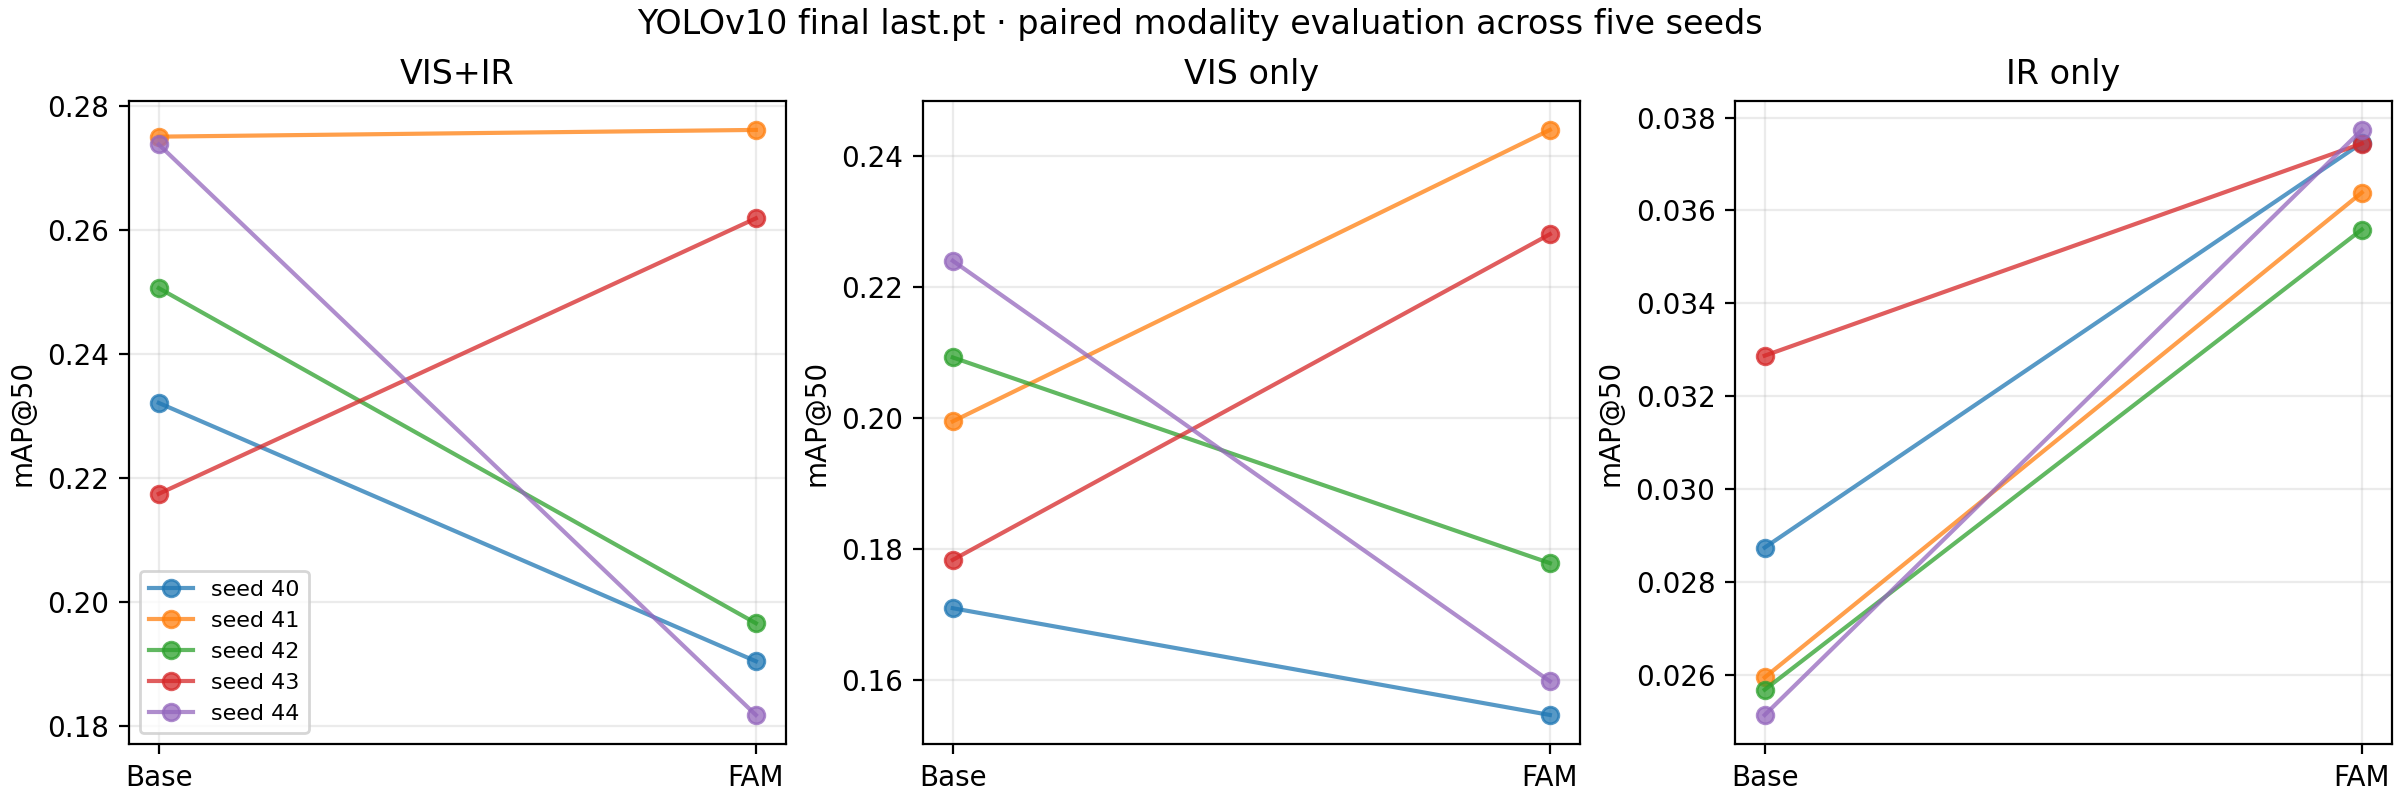
\includegraphics[width=\textwidth]{images/yolov10_final_modality_paired_map50.png}
  \caption{Final YOLOv10 paired modality evaluation. The favorable but very
  small IR-only delta does not compensate for the negative fusion result.}
  \label{fig:yolo-modalities}
\end{figure}

The standalone evaluator produced VIS+IR AP values systematically about
0.0010--0.0021 above the automatic Ultralytics validator. The maximum difference
exceeded the predefined 0.002 sanity tolerance by 0.000077. The tolerance was
not changed. Since all standalone modality conditions use the same evaluator
and the checkpoint ranking is preserved, standalone values are used for the
modality comparison while the automatic table remains the primary training
result.

\subsection{Training-horizon interpretation}

At seed 42, the historical early Base checkpoint obtained 0.3469 at epoch
16 and the historical FAM checkpoint 0.2965 at epoch 89, compared with 0.2494
and 0.1947 at epoch 200. Base YOLOv10 training losses and learning rate match the
old run exactly until its early stop, after which the final run continues.
Training losses keep decreasing while the final test score is lower than the
historical early score.

This pattern is compatible with late overfitting or specialization to the
training sessions, but training loss alone does not establish the cause. The
valid conclusion is that the declared 200-epoch protocol yields a negative FAM
transfer result. A new YOLO study would first require a representative
validation set constructed only from training sessions and a checkpoint rule
fixed before observing MtErie.

\section{Cross-architecture summary}

The three extension families provide different strengths of evidence.
Deformable DETR shows an exploratory increase in median VIS+IR from 0.249 to
0.294 when FAM is added, but its intervals overlap and its protocol predates
the final controls. Complete DINO base is weak under the studied configuration,
so FAM is not tested on that implementation. YOLOv10 uses a final paired-seed
protocol and shows a negative mean FAM effect.

The thesis therefore does not demonstrate positive architectural
transferability. It demonstrates that the FAM concept can be implemented in
multiple detector families, that a promising exploratory trend exists in one,
and that the controlled YOLOv10 transfer does not reproduce the RT-DETR gain.
